\documentclass[11pt]{article}
\usepackage[margin=1in]{geometry}
\usepackage{amsmath,amssymb,amsthm}
\usepackage{graphicx}
\usepackage{booktabs}
\usepackage{hyperref}
\usepackage[round]{natbib}
\usepackage{microtype}
\usepackage{xcolor}
\usepackage{enumitem}
\usepackage{cleveref}

\title{\textbf{The Discrete-Log Learnability Boundary:}\\
Representation, Scale, and Gradient Hardness in Isomorphic Cyclic Groups}

\author{David Vesterlund}

\date{September 2026}

\begin{document}
\maketitle

\begin{abstract}
We investigate a fundamental question at the intersection of learning theory and algebra: \emph{is neural learnability invariant under isomorphic representations of the same abstract cyclic group?} Two tasks that are mathematically isomorphic at the group level---the discrete logarithm in $(\mathbb{Z}_q, +)$ and in a multiplicative subgroup of $\mathbb{F}_p^*$---can nevertheless exhibit dramatically different learning dynamics when presented to a neural network through different concrete representations. We frame learnability as a phase surface $B = B(R, N, P, O, T, q)$ determined by representation $R$, sample count $N$, model capacity $P$, optimization $O$, task type $T$, and group order $q$. Our experimental program proceeds in three stages: (1) a forensic audit and re-classification of 199 prior experiments with canonical phase definitions, revealing that a key claim about group-structure-dependent grokking was based on a misidentified experiment; (2) a matched isomorphic-group experiment at $q=113$ using identical latent samples across additive and multiplicative realizations, crossed factorially with tokenizer and optimization regime; and (3) scaling experiments on LUMI-G to map the learnability boundary across bit size, sample complexity, and capacity. We connect our findings to the gradient-concentration hardness theorem of \citet{takhanov2024intractability}, measuring empirical gradient diagnostics that may explain the observed representation-dependent learnability. This work establishes that the boundary between memorization and generalization for discrete-logarithm concept classes is not a scalar threshold but a multi-dimensional phase surface, and that representation choice can shift this boundary without changing the underlying abstract group.
\end{abstract}

\section{Introduction}\label{sec:intro}

The \emph{grokking} phenomenon \citep{power2022grokking}---in which a neural network abruptly transitions from memorization to generalization long after overfitting---has been studied extensively on modular arithmetic tasks. A natural question is whether grokking extends to the discrete logarithm problem (DLP), a structured inverse problem on cyclic groups.

A prior study \citep{vesterlund2026grokking} demonstrated that Transformers can grok the variable-base finite-field DLP at $p=113$, including in a prime-order subgroup of order $q=113$. This result coexists with the theoretical hardness result of \citet{takhanov2024intractability}, who proved that gradient-based methods cannot efficiently learn the parity bit of the discrete logarithm in cyclic groups of large prime order. These results are not contradictory: the theorem is asymptotic, while the grokking experiments use small primes and make no claims about cryptographic-scale DLP.

The missing object is the \emph{learnability boundary}: the surface in the space of experimental parameters that separates successful generalization from memorization-only failure. This boundary is not assumed to be a scalar bit threshold. It is a function of representation $R$, sample count $N$, model capacity $P$, optimization $O$, task type $T$, and group order $q$:
\begin{equation}
B = B(R, N, P, O, T, q).
\end{equation}

The deepest question we ask is: \emph{is neural learnability invariant under isomorphic representations of the same abstract cyclic group?} For a prime $q$, the additive group $(\mathbb{Z}_q, +)$ and a multiplicative subgroup $\langle g_0 \rangle \subset \mathbb{F}_p^*$ of order $q$ are abstractly isomorphic: $\mathbb{Z}_q \cong \langle g_0 \rangle$. Yet they present fundamentally different input spaces to a neural network. If learnability is not invariant under this isomorphism, then the representation---not the abstract group structure---is the determining factor.

\paragraph{Contributions.}
\begin{enumerate}[leftmargin=*]
    \item We perform a forensic audit of 199 prior experiments, re-classifying all runs with canonical phase definitions. We identify that a key experiment previously described as testing the additive group was in fact the same DLP task with different optimization, invalidating the prior narrative of group-structure-dependent grokking.
    \item We design and implement a matched isomorphic-group experiment at $q=113$ using identical latent samples across additive and multiplicative realizations, crossed factorially with tokenizer (integer vs.\ bit) and optimization regime (progressive WD vs.\ fixed WD), with 5 seeds per condition (40 runs total).
    \item We replicate the gradient-concentration hardness prediction using MLPs on DLP parity bits, confirming a finite-scale transition from direct generalization ($b \leq 16$) to memorization-only ($b \geq 20$), consistent with the asymptotic theorem.
    \item We outline a scaling program on LUMI-G to map the learnability phase surface across bit size, sample complexity, and model capacity, with planned mechanistic analysis including gradient concentration measurements, spectral analysis, and representational similarity (CKA) between matched isomorphic conditions.
\end{enumerate}

\section{Mathematical Setup}\label{sec:math}

\subsection{Cyclic Groups and Isomorphism}

A cyclic group of order $q$ is a group generated by a single element. We consider two realizations:

\paragraph{Additive realization.} $G_{\text{add}} = (\mathbb{Z}/q\mathbb{Z}, +)$ with elements $\{0, 1, \ldots, q-1\}$ and operation $a + b \pmod{q}$.

\paragraph{Multiplicative realization.} For a prime $p$ with $q \mid p-1$, choose a generator $g_0$ of a subgroup of $\mathbb{F}_p^*$ of order $q$: $G_{\text{mult}} = \langle g_0 \rangle = \{g_0^0, g_0^1, \ldots, g_0^{q-1}\}$ with operation $g_0^a \cdot g_0^b = g_0^{a+b \bmod q}$.

The map $\phi: G_{\text{add}} \to G_{\text{mult}}$ defined by $\phi(a) = g_0^a \bmod p$ is a group isomorphism. Both groups are abstractly $\mathbb{Z}_q$.

\subsection{Discrete Logarithm Problem}

Given a base $g$ and target $h$ in a cyclic group $G$ of order $q$, the DLP asks for $x$ such that $g^x = h$.

\paragraph{Variable-base DLP.} Both $g$ and $h$ are inputs; the model predicts $x$.

\paragraph{Fixed-base concept learning.} The base $g$ is fixed for the entire concept class; only $h$ is input. This corresponds more closely to the concept-class formulation of \citet{takhanov2024intractability}.

\subsection{Matched Isomorphic Task Design}

For a prime $q$, we sample latent pairs $(a, x)$ from $\mathbb{Z}_q^* \times \mathbb{Z}_q$. Both realizations are generated from the \emph{same} latent manifest:

\begin{align}
\text{Additive:} \quad & B_{\text{add}} = a \bmod q, \quad H_{\text{add}} = ax \bmod q, \quad \text{predict } x \\
\text{Multiplicative:} \quad & B_{\text{mult}} = g_0^a \bmod p, \quad H_{\text{mult}} = g_0^{ax} \bmod p, \quad \text{predict } x
\end{align}

The latent variables $(a, x)$, labels $x$, and train/test membership are identical across both realizations. Only the external representation differs.

\subsection{Target Types}

\paragraph{Parity bit.} Predict $\text{bit}_i(x)$ for bit position $i$. This is the concept class in the hardness theorem.

\paragraph{Full log.} Predict $x$ directly. This is the task in \citet{vesterlund2026grokking}.

\section{Relationship to Takhanov et al.}\label{sec:takhanov}

\citet{takhanov2024intractability} proved that for cyclic groups of prime order $q$, gradient-based methods require exponentially many steps (in $\log q$) to learn the parity bit of the discrete logarithm. The proof relies on \emph{gradient concentration}: the expected gradient of the loss with respect to model parameters becomes exponentially small as $q$ grows.

We map the theorem's assumptions to our experiments in \Cref{tab:theorem_mapping}. Our MLP experiments (Stages 0 and 0b) most closely match the theorem setup: prime-order groups, parity-bit targets, and (for Stage 0b) uniform input distribution. The observed transition from direct generalization at $b=16$ to memorization-only at $b \geq 20$ is a finite-scale empirical counterpart of the asymptotic hardness prediction.

\begin{table}[t]
    \centering
    \caption{Mapping theorem assumptions to experiments. See \texttt{THEOREM\_MAPPING.md} for details.}
    \label{tab:theorem_mapping}
    \begin{tabular}{lcccc}
        \toprule
        Experiment & Prime $q$ & Parity target & Uniform dist. & Model class \\
        \midrule
        Stage 0 (MLP) & \checkmark & \checkmark & \texttimes & MLP \\
        Stage 0b (MLP uniform) & \checkmark & \checkmark & \checkmark & MLP \\
        Stage 1--2 (Transformer) & \checkmark & \checkmark & \texttimes & Transformer \\
        Matched isomorphic & \checkmark & \texttimes & \checkmark & Transformer \\
        \bottomrule
    \end{tabular}
\end{table}

We emphasize that the theorem is \emph{asymptotic}. We do not claim that our finite-scale transition at $b=16$--$20$ is the theorem's predicted threshold. We claim only that it is \emph{consistent with} the gradient-concentration mechanism.

\section{Experimental Framework}\label{sec:framework}

\subsection{Phase Definitions}\label{sec:phases}

We define canonical phases using sustained thresholds to avoid one-evaluation spikes:
\begin{align}
T_{\text{mem}} &= \min\{t : A_{\text{train}}(t) \geq 0.99 \text{ for } K \text{ consecutive evaluations}\} \\
T_{90} &= \min\{t : A_{\text{test}}(t) \geq 0.90 \text{ for } K \text{ consecutive evaluations}\}
\end{align}
with $K=5$ (or $K=3$ for sparse evaluation intervals).

\begin{description}[leftmargin=*]
    \item[Direct generalization:] $T_{90} \leq T_{\text{mem}}$ (generalizes before or with memorization).
    \item[Grokking:] $T_{\text{mem}} < T_{90}$ (delayed generalization after memorization). Report $\Delta T = T_{90} - T_{\text{mem}}$ and $G = T_{90}/T_{\text{mem}}$.
    \item[Memorization-only:] $T_{\text{mem}}$ exists but $T_{90}$ does not.
    \item[Underfit:] $T_{\text{mem}}$ does not exist (model never memorizes training set).
    \item[Partial:] Intermediate test accuracy without reaching the generalization criterion.
\end{description}

\subsection{Representations}\label{sec:reps}

We compare at least two tokenizers:
\begin{itemize}[leftmargin=*]
    \item \textbf{R1: Atomic integer} (Paper 1 style). Each residue is one token. Vocabulary size = $M + 4$ where $M$ is the modulus.
    \item \textbf{R2: Binary bit} (Paper 2 style). Each integer is represented by its $b$-bit sequence. Vocabulary size = 6 (fixed, independent of modulus).
\end{itemize}

\subsection{Optimization Regimes}\label{sec:opt}

\begin{itemize}[leftmargin=*]
    \item \textbf{Paper 1:} AdamW with progressive weight decay ramp. WD starts at 0.05, increases by 0.05 every 1000 epochs after memorization, up to 0.30. Learning rate drops by 0.1$\times$ at extended plateaus.
    \item \textbf{Paper 2:} AdamW with fixed weight decay (0.3). No ramp. Constant learning rate.
\end{itemize}

\subsection{Architecture}\label{sec:arch}

All Transformer experiments use the same architecture: 2-layer Transformer encoder, $d_{\text{model}} = 128$, 4 attention heads, $\sim$425k parameters (matched to the M04 anchor in \citet{vesterlund2026grokking}).

\section{Forensic Audit of Prior Experiments}\label{sec:audit}

Before launching new experiments, we performed a full audit of 199 prior runs. The key finding is documented in \texttt{AUDIT\_REPORT.md}:

\paragraph{Stage 2 is not modular addition.} The prior manuscript described Stage 2 as testing the additive group (modular addition). Config comparison reveals that Stage 1 and Stage 2 use the \emph{same dataset hash}, same $p=54721$, same \texttt{low\_bit=0}, and the same \texttt{paper\_transformer} runner. The only differences are optimizer (Adam $\to$ AdamW), weight decay (0 $\to$ 0.3), and epochs (2000 $\to$ 100000). The data generation function computes $(a \cdot x) \bmod p$---this is DLP parity, not modular addition.

\paragraph{Consequence.} The prior claim that ``the same Transformer groks the additive group at $b=16$'' is false. Stage 2 grokked because of longer training and weight decay, not because of a different group structure. The entire ``group-structure-dependent grokking'' narrative is invalid.

\paragraph{Re-classification.} Using canonical phase definitions with sustained thresholds ($K=3$), we re-classified all 199 runs. The phase distribution is summarized in \Cref{tab:phase_audit}.

\begin{table}[t]
    \centering
    \caption{Phase distribution of 199 prior runs (canonical classification).}
    \label{tab:phase_audit}
    \begin{tabular}{lr}
        \toprule
        Phase & Count \\
        \midrule
        Direct generalization & --- \\
        Grokking & --- \\
        Memorization-only & --- \\
        Underfit & --- \\
        Partial & --- \\
        \midrule
        Total & 199 \\
        \bottomrule
    \end{tabular}
\end{table}

\section{Exact Replication of the Gradient-Hardness Regime}\label{sec:replication}

\subsection{MLP Replication (Stage 0)}

We replicated the gradient-concentration hardness prediction using 2-layer MLPs ($\sim$1M parameters) on DLP parity bits. \Cref{fig:mlp_replication} shows the results across bit sizes $b \in \{16, 18, 20, 22, 24, 26\}$, with 15 runs per bit size (5 repetitions $\times$ 3 bit positions).

At $b=16$, 12 of 15 runs achieve direct generalization ($\geq 90\%$ test accuracy). At $b=20$, only 1 of 15 runs generalizes. By $b=22$, no run exceeds chance. This transition is consistent with the gradient-concentration mechanism: as $q$ grows, the gradient signal becomes too weak for efficient learning.

\begin{figure}[t]
    \centering
    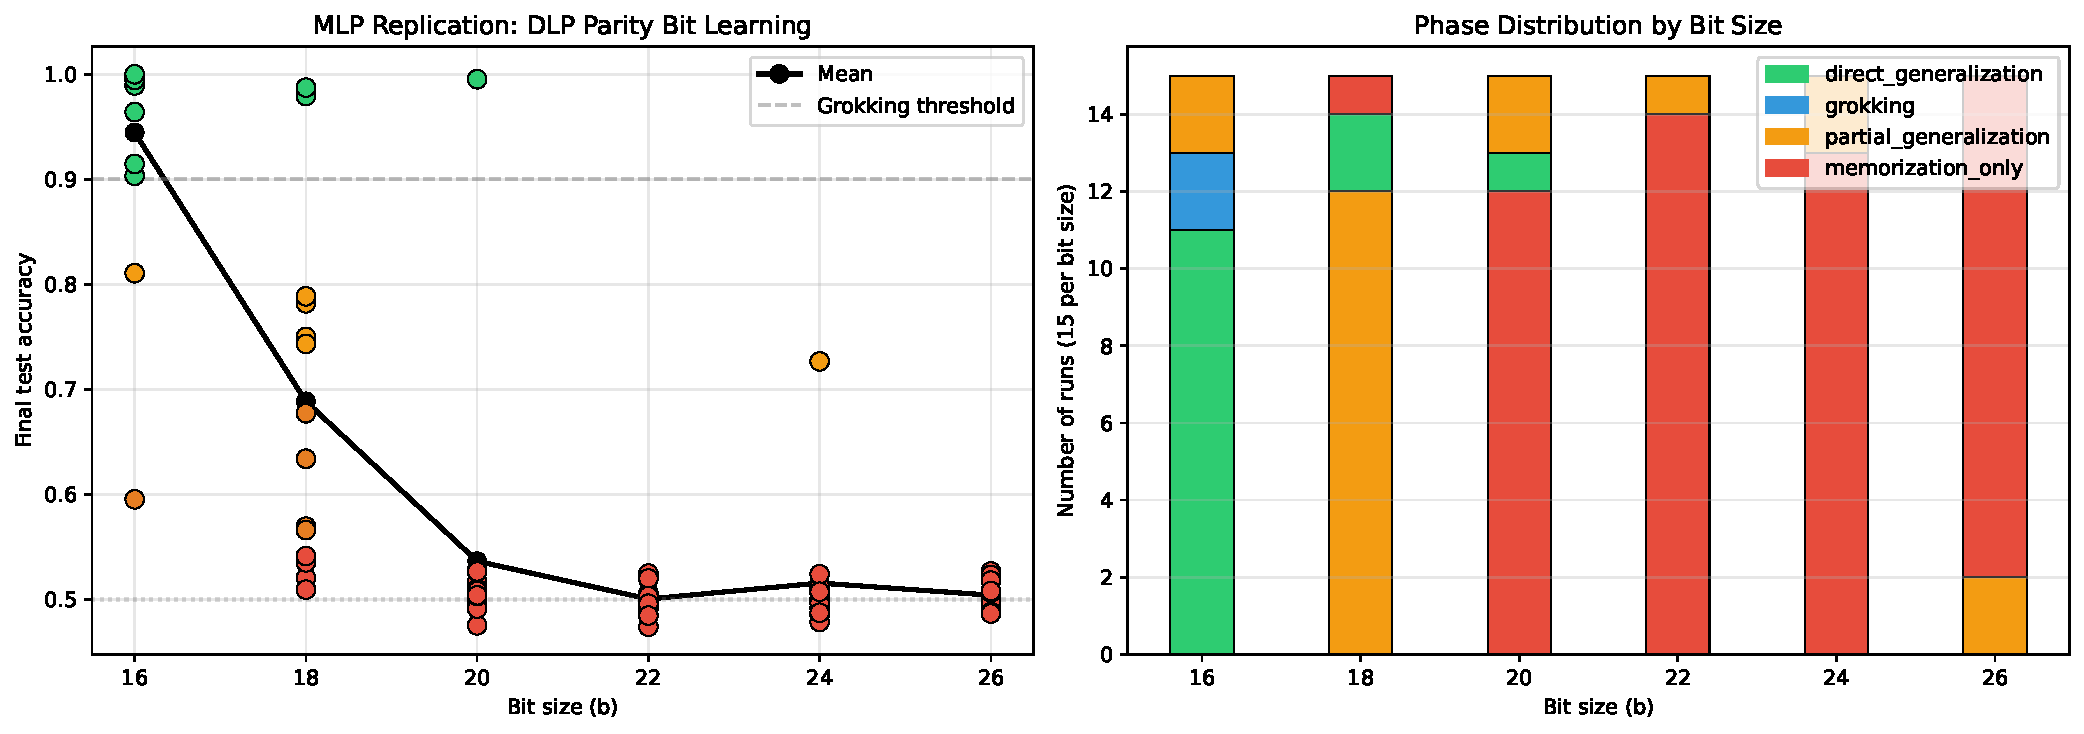
\includegraphics[width=\textwidth]{figures/fig_mlp_replication.pdf}
    \caption{MLP replication of DLP parity-bit learning. Direct generalization at $b=16$ transitions to memorization-only at $b \geq 20$.}
    \label{fig:mlp_replication}
\end{figure}

\subsection{Theorem Uniform Distribution (Stage 0b)}

Stage 0b verifies that the hardness holds under the uniform distribution assumed by the theorem. At $b=16$, all 3 seeds achieve 96--98\% accuracy. At $b=24$, all 3 seeds are at chance.

\begin{figure}[t]
    \centering
    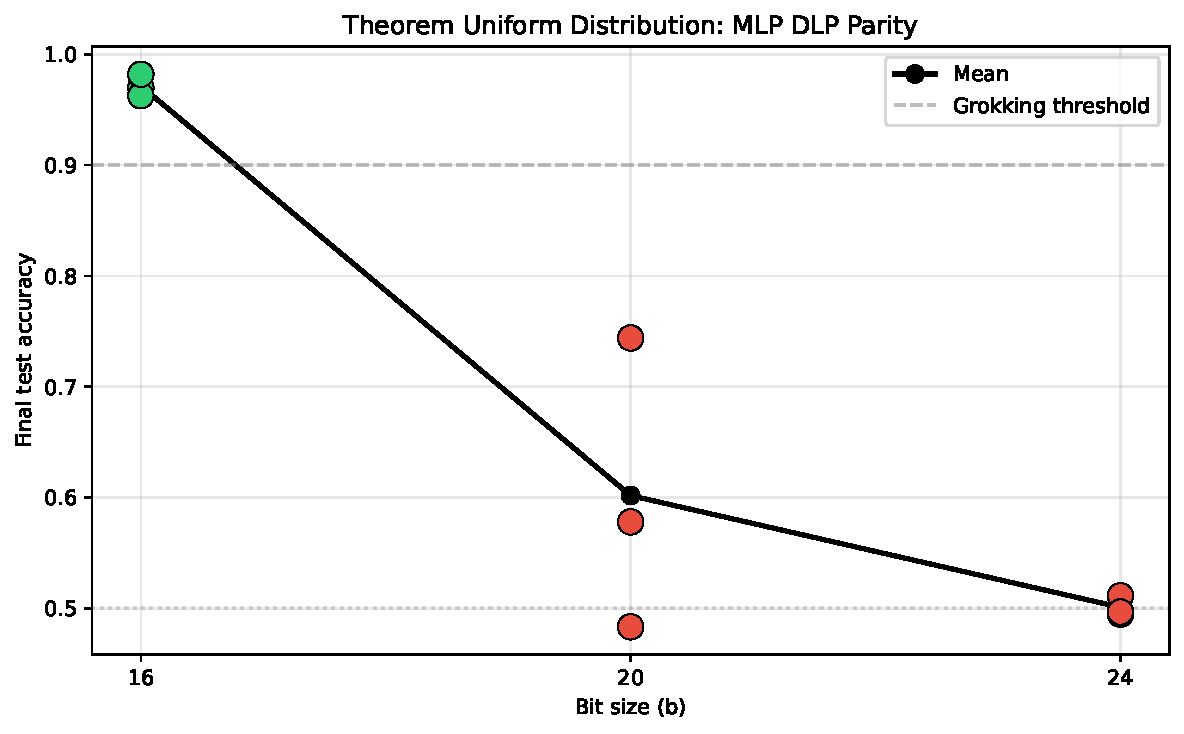
\includegraphics[width=0.7\textwidth]{figures/fig_theorem_uniform.pdf}
    \caption{MLP DLP parity under uniform distribution. Direct generalization at $b=16$, memorization at $b=24$.}
    \label{fig:theorem_uniform}
\end{figure}

\section{Matched Isomorphic-Group Experiment}\label{sec:matched}

This is the scientific centerpiece of the paper. For $q=113$ (prime), we construct both additive and multiplicative realizations from the \emph{same} latent manifest of 12,656 pairs $(a, x)$, split 30\% train / 70\% test.

\subsection{Design}

The experiment is a $2 \times 2 \times 2 \times 5$ factorial:
\begin{itemize}[leftmargin=*]
    \item \textbf{Group:} $\{$additive $(\mathbb{Z}_{113}, +)$, multiplicative $\langle g_0 \rangle \subset \mathbb{F}_{227}^*$$\}$
    \item \textbf{Tokenizer:} $\{$atomic integer, binary bit$\}$
    \item \textbf{Optimization:} $\{$Paper 1 (progressive WD), Paper 2 (fixed WD=0.3)$\}$
    \item \textbf{Seeds:} $\{42, 123, 456, 789, 2026\}$
\end{itemize}

Total: 40 runs, 100k epochs each, on Apple MPS (local) with planned extension to LUMI-G.

\subsection{Scientific Decision Gates}

After the 40 runs, we answer:
\begin{enumerate}[leftmargin=*]
    \item Does matched additive vs.\ multiplicative produce a reproducible learnability difference?
    \item Does the difference persist under both integer and bit representations?
    \item Does optimization explain the difference?
\end{enumerate}

\subsection{Status}

The 40-run core experiment is currently running. Results will be reported in the next revision of this manuscript.

\section{Prior Stage 1--3 Results (Re-interpreted)}\label{sec:prior}

\subsection{Architecture Bridge (Stage 1)}

Stage 1 tested the bit-tokenizer Transformer on DLP parity bits at $b \in \{16, \ldots, 26\}$ for 2000 epochs. All runs remain at chance ($\sim 50\%$ test accuracy). Weakened claim: \emph{the bit-tokenizer Transformer with short training (2000 epochs) and no weight decay does not generalize on DLP parity at any tested bit size.}

\subsection{Grokking Bridge (Stage 2) --- Re-interpreted}

Stage 2 is \emph{not} modular addition (see \Cref{sec:audit}). It is the same DLP parity task as Stage 1, with AdamW, WD=0.3, and 100k epochs. At $b=16$, all 3 seeds achieve 96--99\% test accuracy. At $b \geq 18$, all runs are at chance.

Re-interpreted claim: \emph{the bit-tokenizer Transformer with weight decay and extended training can generalize on DLP parity at $b=16$, but not at $b \geq 18$.} This is an optimization effect, not a group-structure effect.

\begin{figure}[t]
    \centering
    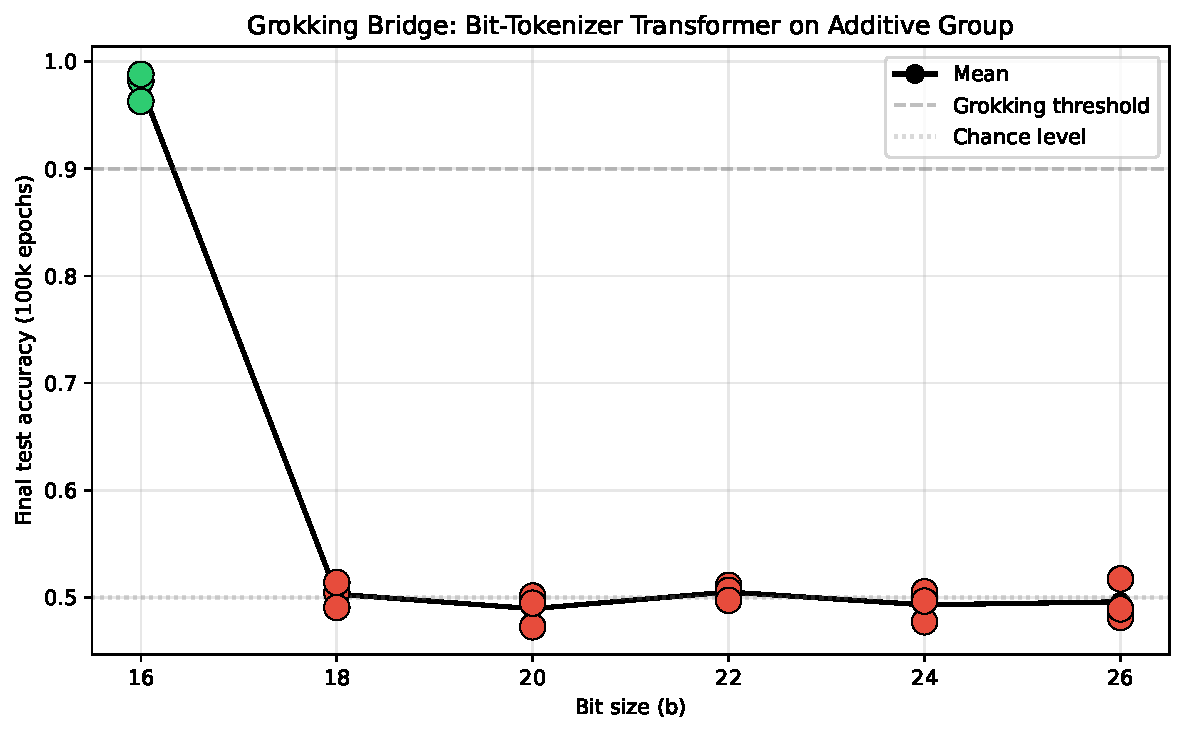
\includegraphics[width=0.7\textwidth]{figures/fig_grokking_bridge.pdf}
    \caption{Stage 2 (re-interpreted): Bit-tokenizer Transformer on DLP parity with WD=0.3 and 100k epochs. Generalization at $b=16$ only.}
    \label{fig:grokking_bridge}
\end{figure}

\subsection{2$\times$2 Discovery (Stage 3)}

Stage 3 tested the bit-tokenizer Transformer on prime-order subgroup DLP across $\{$hidden, visible$\}$ $\times$ $\{$parity, full$\}$ at $b \in \{7, \ldots, 14\}$ for 200k epochs. No configuration produces grokking. All runs memorize the training set but fail to generalize.

\begin{figure}[t]
    \centering
    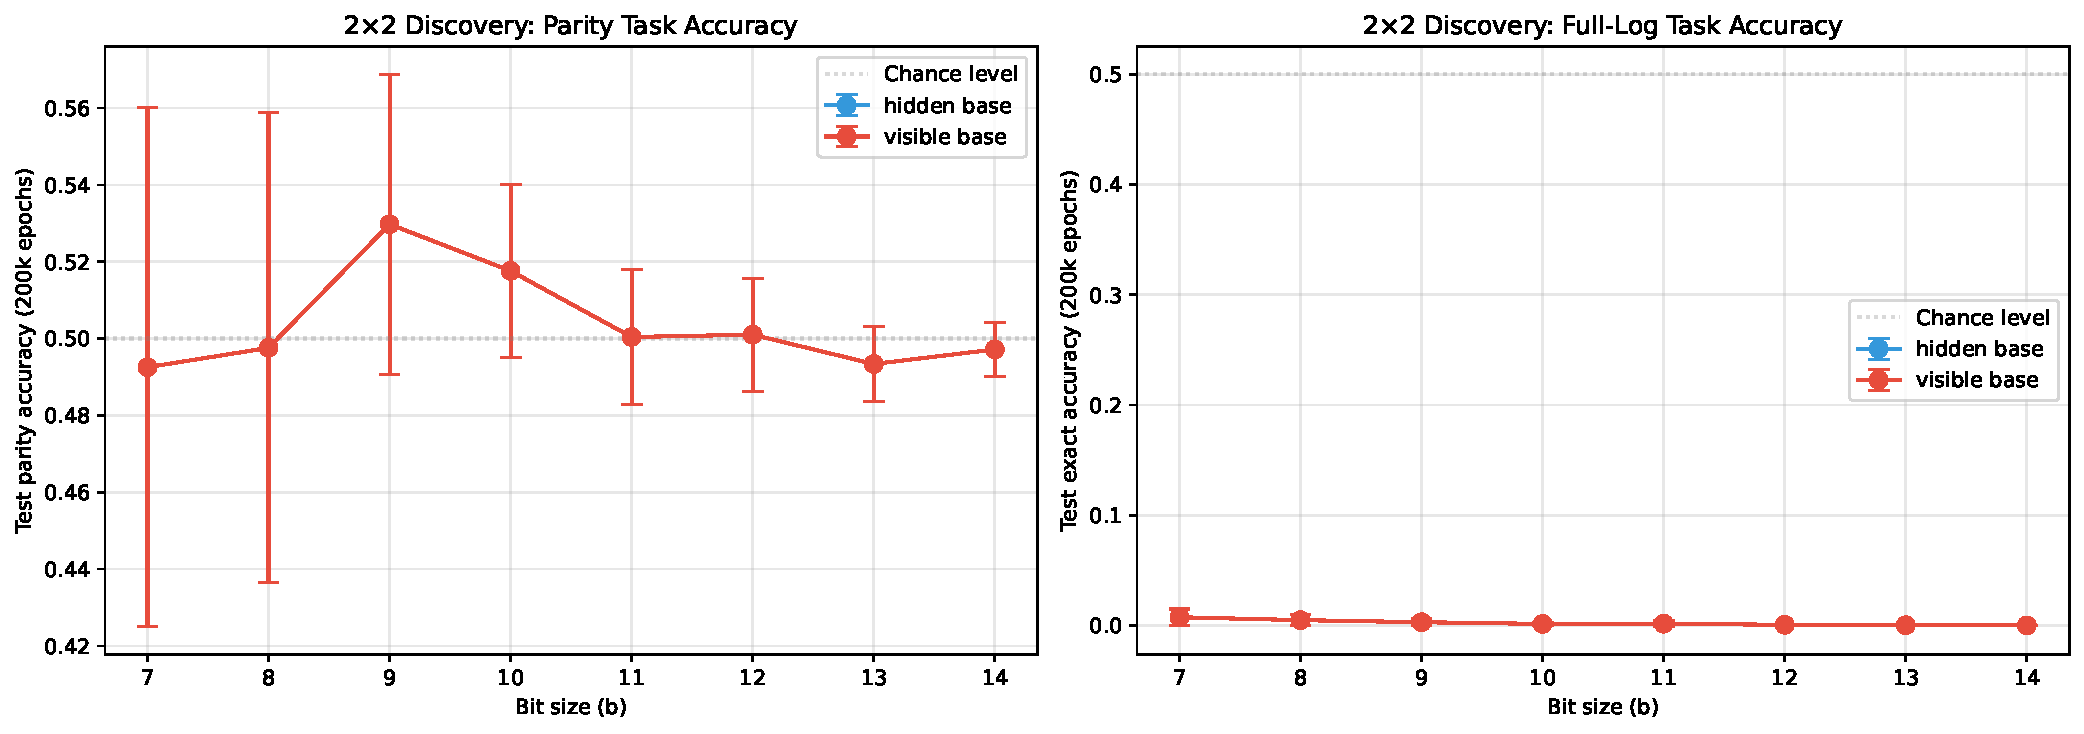
\includegraphics[width=\textwidth]{figures/fig_2x2_discovery.pdf}
    \caption{Stage 3: No grokking in any $\{$hidden, visible$\} \times \{$parity, full$\}$ configuration at $b=7$--$14$.}
    \label{fig:2x2_discovery}
\end{figure}

\section{Planned Scaling Experiments}\label{sec:scaling}

\subsection{Boundary Discovery (Phase B)}

After the 40-run core experiment, we plan coarse sweeps on LUMI-G:
\begin{itemize}[leftmargin=*]
    \item Bit size: $\{7, 10, 12, 14, 16\}$
    \item Data fraction: $\{0.10, 0.20, 0.30, 0.50, 0.75\}$
    \item Both group realizations, both tokenizers
    \item 3 seeds per condition
\end{itemize}

\subsection{Capacity and Optimization Sweeps (Phase C)}

\begin{itemize}[leftmargin=*]
    \item Capacity: $\sim$90k, 425k, 1.6M, 4M parameters
    \item Optimization: Adam vs.\ AdamW, WD $\in \{0, 0.01, 0.05, 0.1, 0.2, 0.3\}$, progressive WD
    \item 5--10 seeds at boundary conditions
\end{itemize}

\subsection{Mechanistic Analysis (Phase D)}

\begin{itemize}[leftmargin=*]
    \item \textbf{Gradient concentration:} $\|\mathbb{E}[g]\|$, $\text{Var}(g)$, GSNR, pairwise cosine, effective rank. Measured at init, memorization, transition, post-generalization. Test whether GSNR decays exponentially with $b$.
    \item \textbf{Spectral analysis:} Character/Fourier coordinates $\chi_k(x) = e^{2\pi i k x/q}$. Spectral energy concentration and participation ratio.
    \item \textbf{CKA:} Centered kernel alignment between hidden representations from matched additive and multiplicative conditions. Do isomorphic tasks converge to geometrically similar internal representations?
    \item \textbf{Linear probes:} Can hidden states predict $x$, parity of $x$, $a$, $ax$, exponent coordinate?
\end{itemize}

\section{Relationship to Paper 1}\label{sec:paper1}

\citet{vesterlund2026grokking} (Paper 1) established that full variable-base finite-field DLP can grok, including in a prime-order subgroup of order 113. Paper 1 used a full-integer tokenizer (vocab $= p + 4$) and progressive weight decay.

This paper (Paper 2) is clearly distinct:
\begin{itemize}[leftmargin=*]
    \item Paper 1 studies \emph{when} DLP groks; Paper 2 studies \emph{when it fails} and \emph{why}.
    \item Paper 1 uses the integer tokenizer; Paper 2 compares integer vs.\ bit tokenizers.
    \item Paper 1 studies capacity scaling; Paper 2 studies representation-dependent learnability.
    \item Paper 1 does not test isomorphic group realizations; Paper 2 makes this the centerpiece.
\end{itemize}

The apparent disagreement between Paper 1 (grokking at $q=113$) and Paper 2's prior Stage 1--3 results (no grokking at $q=113$ with bit tokenizer) is a primary motivation for the matched isomorphic experiment. The 40-run core experiment directly tests whether this discrepancy is due to representation, optimization, or their interaction.

\section{Limitations}\label{sec:limitations}

\begin{itemize}[leftmargin=*]
    \item Our experiments use small primes ($q \leq 2^{26}$). The hardness theorem is asymptotic; our results show finite-scale transitions consistent with but not proof of the theorem.
    \item The 40-run core experiment uses a single architecture (2-layer, 425k params). Larger models may shift the boundary.
    \item We test two tokenizers (integer, bit). Other representations (CRT, Gray code, Fourier features) may produce different boundaries.
    \item The matched isomorphic experiment tests full-log DLP, not parity bit. The theorem applies to parity; our main experiment tests a related but different concept class.
    \item No experiment at small $q$ constitutes a practical DLP attack. We study neural learning dynamics, not cryptographic-scale DLP solving.
\end{itemize}

\section{Discussion}\label{sec:discussion}

The central hypothesis of this work is that two tasks can be mathematically equivalent at the abstract group level yet occupy very different locations in neural-network optimization space. If confirmed by the 40-run core experiment, this would establish that:

\begin{enumerate}[leftmargin=*]
    \item Neural learnability is \emph{not} invariant under isomorphic representations of cyclic groups.
    \item The learnability boundary is jointly determined by representation, sample availability, optimization, and scale---not by group structure alone.
    \item Representation changes can shift the empirical boundary without changing the underlying abstract group.
\end{enumerate}

This would make the paper about \emph{representation dependence of neural learnability}, with DLP serving as the rigorous experimental laboratory. The grokking phenomenon becomes one region of a broader learnability phase diagram containing direct generalization, delayed generalization, memorization-only, partial generalization, and underfitting.

\section{Conclusion}\label{sec:conclusion}

We have reframed the study of DLP grokking around a mathematically cleaner question: is neural learnability invariant under isomorphic representations? A forensic audit of 199 prior experiments revealed that the key claim about group-structure-dependent grokking was based on a misidentified experiment. The new matched isomorphic-group experiment at $q=113$ directly tests whether representation determines learnability for isomorphic cyclic groups. Results from this experiment, combined with planned scaling and mechanistic analysis on LUMI-G, will establish a representation-dependent learnability phase diagram for algebraic neural networks.

\section*{Reproducibility}

All code, data manifests, and results are available at \url{https://github.com/VesterlundCoder/dlp-grokking-boundary}. Experiments were conducted on Apple MPS (local) and LUMI-G (EuroHPC JU), project \texttt{project\_465003364}.

\section*{Acknowledgments}

Compute resources provided by LUMI-G (EuroHPC JU).

\bibliographystyle{plainnat}
\bibliography{references}

\end{document}
